
\section{Implementasi Algoritma Paralel pada Library big integer}
\subsection{Lingkungan Implementasi}
Sesuai dengan pertimbangan pada subbab \ref{sec:parallel_env}, implementasi algoritma paralel akan dilakukan dengan kakas ....

tambahin arsitekturnya, openssl+apache
\begin{figure}[h]
  \centering
  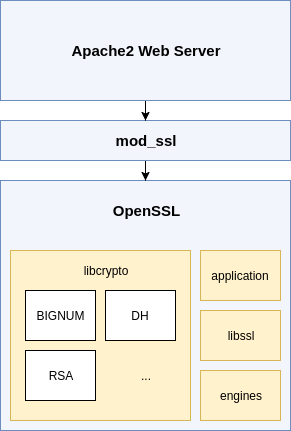
\includegraphics[width=0.4\textwidth]{resources/ch-4/implementation_arch.png}
  \caption{Arsitektur OpenSSL}
  \label{fig:openssl_arch}
\end{figure}

\subsection{Batasan Implementasi}
Fungsi mana yang engga dihandle, kenapa
Batasin cuma di satu ciphertext doang. TLS\_DH\_RSA\_WITH\_AES\_256\_CBC\_SHA256.

\subsection{Struktur Data big integer}
\subsubsection{BIGNUM}
Pada OpenSSL, sebuah big integer direpresentasikan dalam struktur data BIGNUM. BIGNUM terdiri dari sebuah array dengan ukuran dinamis, dengan demikian secara teori BIGNUM tidak memiliki nilai maksimum. Untuk keperluan paralelisasi, BIGNUM dapat digunakan tanpa mengubah strukturnya sedikitpun. BIGNUM sendiri merupakan sebuah \textit{struct} yang memiliki deklarasi sebagai berikut.

\begin{lstlisting}[style = code]
struct bignum_st {
       BN_ULONG *d;
       int top;
       int dmax;
       int neg;
       int flags;
};
\end{lstlisting}

|BN_ULONG| sendiri adalah sebuah makro yang menggantikan |unsigned long| pada komputer 32 bit atau |unsigned long long| pada komputer 64 bit.

|d| adalah pointer untuk array of integer.

|top| merupakan index |d| yang terakhir digunakan plus satu.

|dmax| adalah panjang maksimum array yang telah dibuat. |neg| bernilai satu jika BIGNUM bernilai negatif.

BIGNUM telah memiliki beberapa fungsi primitif yang dapat digunakan untuk membuat, memanipulasi, dan menghancurkan \textit{struct} tersebut. Primitif yang ada adalah seperti berikut.

\begin{lstlisting}[caption=Primitif BIGNUM]
 BIGNUM *BN_new(void);
 void BN_init(BIGNUM *);
 void BN_clear(BIGNUM *a);
 void BN_free(BIGNUM *a);
 void BN_clear_free(BIGNUM *a);
\end{lstlisting}

|BN_new()| akan mengalokasi dan menginisialisasi sebuah struktur BIGNUM.

|BN_init()| menginisialisasi BIGNUM yang sudah ada.

|BN_clear()| mengubah nilai seluruh komponen BIGNUM a (d, top, dmax) menjadi 0. |BN_clear()| dapat digunakan untuk menghapus data sensitif yang sudah tidak digunakan lagi seperti nilai kunci RSA atau AES.

|BN_free()| mengembalikan memori komponen BIGNUM pada sistem.

|BN_clear_free()| mengubah nilai seluruh komponen BIGNUM a menjadi 0 kemudian mengembalikan memori BIGNUM pada sistem.


% Sebutin fungsi yang dipake?
\subsection{Modul Operasi Aritmatika}
snippet code aja pemanggilan
\subsubsection{Modul Penjumlahan}
\subsubsection{Modul Pengurangan}
\subsubsection{Modul Perkalian}
\subsubsection{etc.}
